\documentclass[a4paper]{article}
\usepackage[top=2cm, bottom=2cm, left=2cm, right=2cm]{geometry}
\usepackage[utf8]{inputenc}
\usepackage{subcaption,graphicx}

\title{Compte rendu TP2 Algorithmie}
\author{Léo Combaret}
\date{Mars 2022}

\begin{document}
    %espacement entre les lignes d'un tableau
\renewcommand{\arraystretch}{1.5}
%régler l'espacement entre les lignes
\newcommand{\HRule}{\rule{\linewidth}{0.5mm}}
\maketitle

\section{Partie A}

\subsection{Fonction \emph{creer-graphe}}
Pour cette première question, nous allons implémenter une fonction \emph{creer-graphe} 
qui va prendre en argument le nom d'un fichier sans l'extension $.txt$ ainsi q'une booléenne qui indique si le 
graphe est orienté ou pas.\\

De plus, nous voulons que cette fonction renvoie un $Graphe$ donc nous avons construit dans notre fichier head
une structure de type $Graphe$ qui contient entr'autres un tableau qui va contenir des listes chainés. De ce fait
nous allons aussi implémenter une structure de type $liste$.\\

Ensuite, nous allons donc récupérer les deux premières informations du fichiers qui sont le nombre de sommets et d'aretes
que nous allons stocker dans leur variable respective.\\

Après cela, on initialise et vide nos tableaux $adj$ et $visited$.\\
Et enfin, on récupère le premier sommet et le deuxième sommet pour chaque ligne jusqu'à la fin du fichier.
Si le graph est orienté on va rajouter le sommet 2 dans la liste des adjacents du sommet 1. Sinon les deux sont rajoutés dans 
leur liste respective d'adjacents.\\

Nous avons créé des fonctions \emph{print-liste} et \emph{print-graphe} pour pouvoir visualiser les différentes listes du tableau ainsi que 
des fonctions \emph{free-liste} et \emph{free-graphe} pour libérer les allocations d'espace.\\
\HRule 
\begin{figure*}[htp]
    \centering
    \begin{subfigure}{0.45\textwidth}
      \centering
      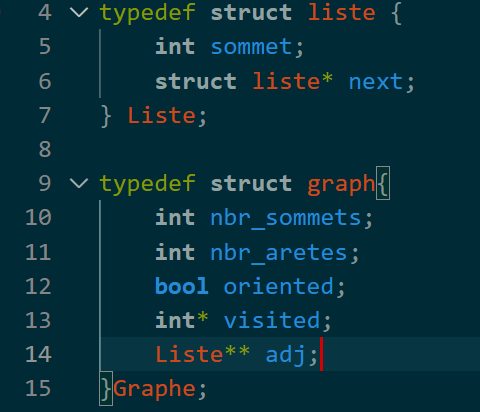
\includegraphics[width=3cm]{./Photos/Structures.png}
      \caption{}
    \end{subfigure}%
    \hfill
    \begin{subfigure}{0.45\textwidth}
      \centering
      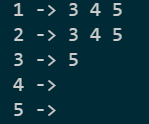
\includegraphics[width=3cm]{./Photos/print_graphe.png}
      \caption{}
    \end{subfigure}
  \caption { (a) Structures (b) Affichage du graphe retourné pour le graph-1}
\end{figure*}

\subsection{Fonction \emph{creer-dot}}
Pour cette seconde question, nous allons implémenter une fonction $creer-dot()$ 
qui va prendre en argument le nom d'un fichier sans l'extension $.txt$ ainsi q'une booléenne qui indique si le 
graphe est orienté ou pas.\\

Pour cela, nous allons créer un fichier $.dot$ du même nom dans lequel on va y écrire nos instructions.
Si le graphe est orienté, on va commencer le fichier par \emph{digraph G}, sinon par \emph{graph G}\\
Ensuite nous allons lire le sommet 1 et 2 pour chaque connexion et les écrire sur le fichier \emph{.dot}
Ces deux sommets sont reliés par une flèche si orientés, par deux traits si non.\\
Ainsi la fonction renvoie un fichier $.dot$ qui va pouvoir permettre à \emph{graphviz} de le lire.\\  
\hfill
\begin{figure*}[htp]
    \centering
    \begin{subfigure}{0.225\textwidth}
      \centering
      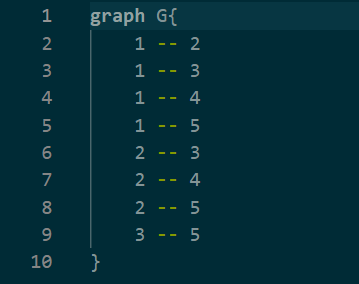
\includegraphics[width=3cm]{./Photos/dot_non_oriente.png}
      \caption{}
    \end{subfigure}%
    \hfill
    \begin{subfigure}{0.225\textwidth}
      \centering
      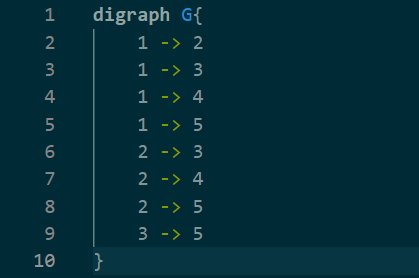
\includegraphics[width=3cm]{./Photos/dot_oriente.png}
      \caption{}
    \end{subfigure}%
    \hfill
    \begin{subfigure}{0.225\textwidth}
        \centering
        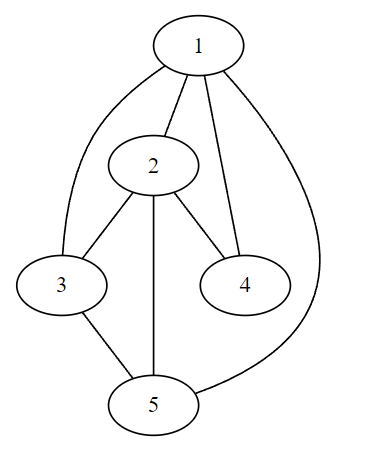
\includegraphics[width=3cm]{./Photos/graphviz_non_oriente.png}
        \caption{}
    \end{subfigure}%
    \hfill
    \begin{subfigure}{0.225\textwidth}
        \centering
        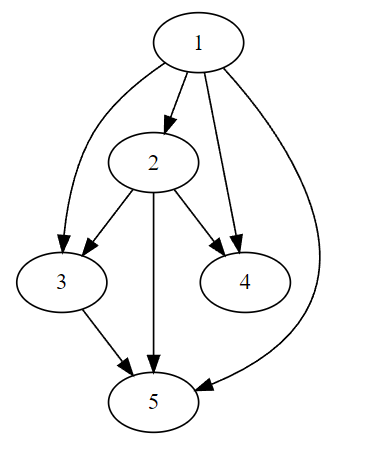
\includegraphics[width=3cm]{./Photos/graphviz_oriente.png}
        \caption{}
    \end{subfigure}
  \caption { (a) .dot non oriente (b) .dot oriente A (c) graphviz non oriente (d) graphviz oriente}
\end{figure*}

\subsection{Fonction \emph{dfs}}
Ici nous allons implémenter un \emph{dfs} qui va prendre en argument le graphe que l'on veut parcourir, ainsi qu'un noeud
duquel partir. Pour cela nous allons utiliser le tableau \emph{visited} du graphe qui nous indique quel sommet a été visité
ou non.\\
Ainsi, nous allons procéder à une itération récursive de la fonction \emph{dfs} jusqu'à ce qu'on ai visité tous les sommets
possible du graphe en partant de ce sommet.\\

\subsection{Fonction \emph{connexity}}
La fonction connexity prend en argument un graphe et renvoie un bool qui nous indique si le graphe est connexe ou pas.\\
La fonction va donc faire un \emph{dfs} à partir d'un sommet pris au hasard. Le \emph{dfs} va mettre à jour le tableau \emph{visited}
du graphe, et si tous les élélemnts de ce tableaux valent 1 i.e que tous les sommets aient été visités, alors le graphe est connexe.\\

\subsection{Fonction \emph{invert}}
La fonction invert prend pour argument un graphe pour retourner l'inverse de ce graphe\\
Pour ce faire, nous allons tout d'abord créer un graphe \emph{inverted} de même nombre de sommet et d'aretes mais d'un tableau de sommet vide.\\
Ensuite, nous allons parcourir le tableau du graphe en argument. Chaque itération va traiter la liste des adjacents du sommet x. 
De ce fait, le sommet x va être ajouté à chaque liste des adjacents de sa propre liste.\\

\section{Axe d'amélioration}
J'ai quelques axes d'amélioration à travailler comme par exemple une incompréhension de non fonctinonement de ma fonction \emph{ajouter()} que 
ne comprends toujours pas. Je pense que j'ai un problème avec \emph{fgets()} que je n'arrive pas à résoudre. Par exemple, pour le graph 3, la fonction
saute les 6 premieres aretes.\\
De plus, ma fonction \emph{invert} ainsi que les fonctions \emph{ajouter} ne s'exectuent pas sans que je \emph{printf()} quelque chose. De plus, la boucle 
se stop après le traitement de la liste du premier noeud et si on fait commencer l'itération à 1, le programme marche.
Je trouve aussi que l'organisation de mon code peut être amélioré avec des commentaires et des classification des fonctions pour y voir plus claire.\\
\hfill
\begin{figure*}[htp]
  \centering
  \begin{subfigure}{0.30\textwidth}
    \centering
    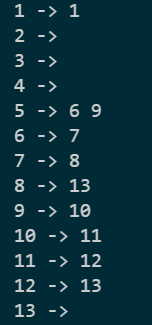
\includegraphics[scale=0.5]{./Photos/Bug_saut.png}
    \caption{}
  \end{subfigure}%
  \hfill
  \begin{subfigure}{0.30\textwidth}
    \centering
    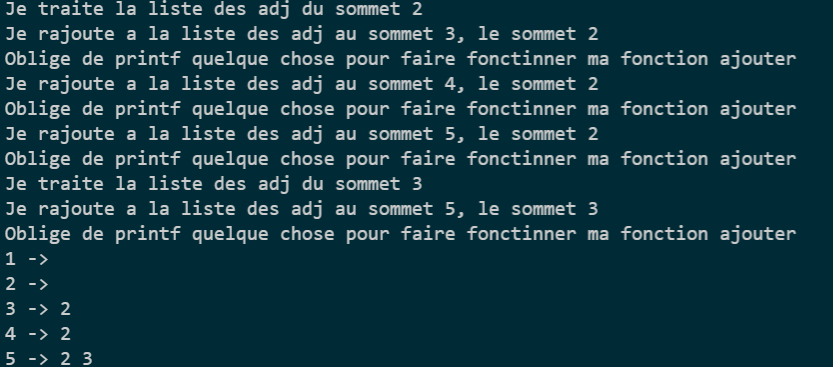
\includegraphics[width=3cm]{./Photos/Invert_bug1.png}
    \caption{}
  \end{subfigure}%
  \hfill
  \begin{subfigure}{0.30\textwidth}
      \centering
      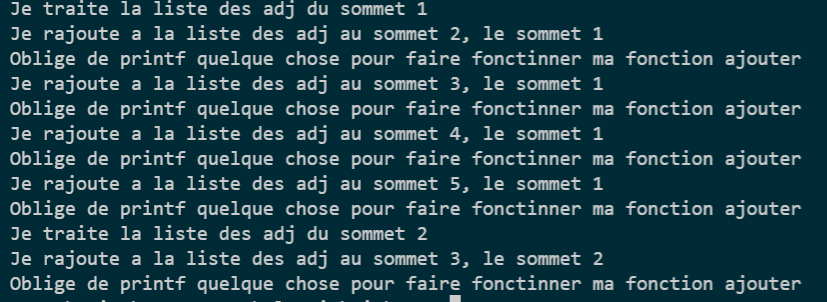
\includegraphics[width=3cm]{./Photos/Invert_bug2.png}
      \caption{}
  \end{subfigure}%
  \hfill
\caption { (a) Graphe du 3 (b) Arret après le premier noeud A (c) Inversé en sautant le premier noeud}
\end{figure*}
\end{document}